\documentclass[11pt]{standalone}
\usepackage{amssymb}
\usepackage{amsmath}
\usepackage[no-math]{fontspec}
\usepackage{unicode-math}
\usepackage{libertinus}
\usepackage{pgf,xcolor}
\usepackage{tikz}
\usetikzlibrary{arrows.meta, backgrounds, calc}
\usepackage{pgfplots}
\pgfplotsset{compat=newest}

\definecolor{my_darkgray}{HTML}{484949}
\definecolor{my_lightgray}{HTML}{F3F4F4}
\definecolor{my_darkblue}{HTML}{005A94}
\definecolor{my_lightblue}{HTML}{CCDEE9}
\definecolor{my_yellow}{HTML}{FFEC7F}
\definecolor{my_red}{HTML}{E60000}
\definecolor{my_orange}{HTML}{E87846}

% Asymptote positions: π/2 ≈ 1.5708, 3π/2 ≈ 4.7124
\newcommand{\pihalf}{1.5708}
\newcommand{\threepi}{4.7124}

\begin{document}
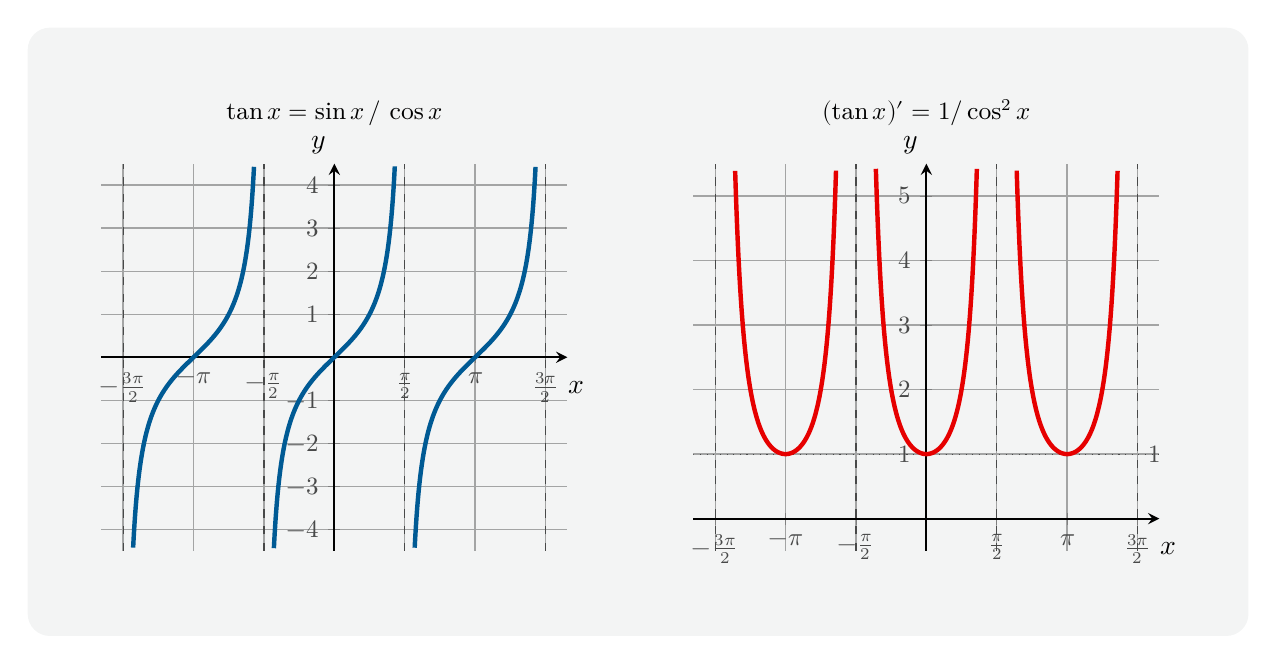
\begin{tikzpicture}[
    show background rectangle,
    background rectangle/.style={fill=my_lightgray, rounded corners=8pt},
    inner frame sep=0.8cm
]

% ── Left plot: tan(x) ───────────────────────────────────────────────────────
% Three continuous branches split at ±π/2 and ±3π/2.
% restrict y to domain guards against residual spike artifacts at the clips.
\begin{axis}[
    name=left plot,
    axis lines = center,
    xlabel = {$x$},
    ylabel = {$y$},
    xlabel style = {at={(axis cs:5.4,0)}, anchor=north, yshift=-5pt},
    ylabel style = {anchor=south east},
    title = {$\tan x = \sin x\,/\,\cos x$},
    title style = {font=\small, text=black, yshift=4pt},
    grid = both,
    grid style = {line width=0.3pt, draw=my_darkgray!30},
    major grid style = {line width=0.5pt, draw=my_darkgray!50},
    % axis equal omitted: y range ±4 vs x range ±5 – equal scaling would
    % flatten the steep branches near the asymptotes
    axis line style = {thick},
    xmin = -5.2, xmax = 5.2,
    ymin = -4.5, ymax = 4.5,
    xtick = {-4.71239, -3.14159, -1.5708, 0, 1.5708, 3.14159, 4.71239},
    xticklabels = {
        $-\tfrac{3\pi}{2}$, $-\pi$, $-\tfrac{\pi}{2}$,
        $0$,
        $\tfrac{\pi}{2}$, $\pi$, $\tfrac{3\pi}{2}$
    },
    ytick = {-4,-3,-2,-1,0,1,2,3,4},
    yticklabel style = {
        /pgf/number format/fixed,
        /pgf/number format/precision=0,
        font=\small,
        text=my_darkgray
    },
    xticklabel style = {font=\small, text=my_darkgray},
    width=7.5cm, height=6.5cm,
    clip=true,
]

% Asymptote dashed lines at x = ±π/2 and ±3π/2
\foreach \xa in {-4.71239, -1.5708, 1.5708, 4.71239}{
    \addplot[draw=my_darkgray, dashed, thin]
        coordinates {(\xa,-4.5) (\xa,4.5)};
}

% Branch 1: (-3π/2, -π/2)
\addplot[draw=my_darkblue, samples=300, ultra thick,
    domain=-4.6624:-1.6308,
    restrict y to domain=-4.5:4.5
]{ tan(deg(x)) };

% Branch 2: (-π/2, π/2)
\addplot[draw=my_darkblue, samples=300, ultra thick,
    domain=-1.5108:1.5108,
    restrict y to domain=-4.5:4.5
]{ tan(deg(x)) };

% Branch 3: (π/2, 3π/2)
\addplot[draw=my_darkblue, samples=300, ultra thick,
    domain=1.6308:4.6624,
    restrict y to domain=-4.5:4.5
]{ tan(deg(x)) };

\end{axis}

% ── Right plot: 1/cos²(x) ───────────────────────────────────────────────────
% 1/cos²(x) ≥ 1 everywhere on its domain; it diverges at the same asymptotes.
% y range starts at 0 to show the minimum value of 1 clearly.
\begin{axis}[
    name=right plot,
    at={($(left plot.east)+(1.6cm,0)$)},
    anchor=west,
    axis lines = center,
    xlabel = {$x$},
    ylabel = {$y$},
    xlabel style = {at={(axis cs:5.4,0)}, anchor=north, yshift=-5pt},
    ylabel style = {anchor=south east},
    title = {$(\tan x)' = 1/\cos^2 x$},
    title style = {font=\small, text=black, yshift=4pt},
    grid = both,
    grid style = {line width=0.3pt, draw=my_darkgray!30},
    major grid style = {line width=0.5pt, draw=my_darkgray!50},
    % axis equal omitted: y range 0..5 vs x range ±5 – would make the
    % parabola-like branches appear nearly flat
    axis line style = {thick},
    xmin = -5.2, xmax = 5.2,
    ymin = -0.5, ymax = 5.5,
    xtick = {-4.71239, -3.14159, -1.5708, 0, 1.5708, 3.14159, 4.71239},
    xticklabels = {
        $-\tfrac{3\pi}{2}$, $-\pi$, $-\tfrac{\pi}{2}$,
        $0$,
        $\tfrac{\pi}{2}$, $\pi$, $\tfrac{3\pi}{2}$
    },
    ytick = {0,1,2,3,4,5},
    yticklabel style = {
        /pgf/number format/fixed,
        /pgf/number format/precision=0,
        font=\small,
        text=my_darkgray
    },
    xticklabel style = {font=\small, text=my_darkgray},
    width=7.5cm, height=6.5cm,
    clip=true,
]

% Asymptote dashed lines at x = ±π/2 and ±3π/2
\foreach \xa in {-4.71239, -1.5708, 1.5708, 4.71239}{
    \addplot[draw=my_darkgray, dashed, thin]
        coordinates {(\xa,-0.5) (\xa,5.5)};
}

% Minimum value line at y = 1
\addplot[draw=my_darkgray, dotted, thin, domain=-5.2:5.2]{ 1 };
\node[anchor=west, font=\small, text=my_darkgray]
    at (axis cs:4.75, 1) {$1$};

% Branch 1: (-3π/2, -π/2)
\addplot[draw=my_red, samples=300, ultra thick,
    domain=-4.6624:-1.6308,
    restrict y to domain=0:5.5
]{ 1 / (cos(deg(x)))^2 };

% Branch 2: (-π/2, π/2)
\addplot[draw=my_red, samples=300, ultra thick,
    domain=-1.5108:1.5108,
    restrict y to domain=0:5.5
]{ 1 / (cos(deg(x)))^2 };

% Branch 3: (π/2, 3π/2)
\addplot[draw=my_red, samples=300, ultra thick,
    domain=1.6308:4.6624,
    restrict y to domain=0:5.5
]{ 1 / (cos(deg(x)))^2 };

\end{axis}

\end{tikzpicture}
\end{document}
